\documentclass[12pt,letterpaper]{article}
\usepackage{amsmath,amsthm,amsfonts,amssymb,amscd}
\usepackage{fullpage}
\usepackage{lastpage}
\usepackage{enumerate}
\usepackage{fancyhdr}
\usepackage{tikz}
\usetikzlibrary{arrows, automata}
\usepackage{mathrsfs}
\usepackage{dsfont}
\usepackage[margin=3cm]{geometry}
\setlength{\parindent}{0.0in}
\setlength{\parskip}{0.05in}

\newcommand\refobj{\textmd{ref}}
\newcommand\prob{\mathbb{P}}
\newcommand\E{\mathbb{E}}
\DeclareMathOperator*{\argmin}{\arg\!\min}

\begin{document}
\section*{Introduction}
Let $\Gamma$ represent the knowledge of the table. $\Gamma$ is composed of $\gamma_1, \ldots, \gamma_n$, corresponding to the objects on the table, and $\gamma_{\textmd{wall}_1}, \gamma_{\textmd{wall}_2}, \gamma_{\textmd{wall}_3}, \gamma_{\textmd{wall}_4}$, corresponding to the four walls (edges) of the table. Each $\gamma$ contains position and dimension information about the object in question.   \\
\\
Let $\lambda$ be the command the user gives, consisting of a distance $\lambda_d$ a direction (relation) $\lambda_r$ and a reference object $\lambda_f$. For the sake of testing this algorithm, we will assume perfect ability to parse the command and extract this information.Therefore we assume there is a perfect correspondence between $\lambda_f$ and $\gamma_\refobj$, where $\gamma_\refobj \in \{\gamma_1, \ldots, \gamma_n\}$. In addition, we assume that the direction is in the set $\{$left, right, in front, behind$\}$ and map $\lambda_r$ to the corresponding direction vectors $\{[1, 0], [-1, 0], [0, 1], [0, -1]\}$  Underlying this assumption is the larger assumption that all commands map to a single direction vector - discussion of how we plan to improve this can be found later in this paper. \\
\\
As an example, if the command is `five inches to the right of the bowl', then we have $\lambda_d = 5$, $\lambda_r = [1, 0]$, $\lambda_f = $ the bowl. \\
\\
Our goal then is to estimate a function $\mathbb{P}(x, y | \lambda, \Gamma)$ which gives the probability that a user was referring to the point $(x, y)$ given the command $\lambda$ and world $\Gamma$. \\
\\
From the command and reference, we calculate a naive mean, which is the point you would select if you went exactly the distance specified by the command, in the direction specified by the command. From this we calculate four features for a log-linear model.



\section*{Feature Calculation}
\subsection{Calculating $\hat{\mu}$}
The naive mean, $\hat{\mu}$, is what is obtained by going exactly the distance specified in the command from the edge of the object. This is calculated as follows:
\[
\hat{\mu} = \begin{cases} \gamma_\refobj.center + \frac{\gamma_\refobj.height}{2} + \lambda_d, & \lambda_r = [0, -1] \\
\gamma_\refobj.center - \frac{\gamma_\refobj.height}{2} - \lambda_d, & \lambda_r = [0, 1] \\
 \gamma_\refobj.center + \frac{\gamma_\refobj.width}{2} + \lambda_d, & \lambda_r = [1, 0] \\
 \gamma_\refobj.center - \frac{\gamma_\refobj.width}{2} - \lambda_d, & \lambda_r = [-1, 0] \end{cases}
\]

\subsection*{Calculating $T_1$ and $T_2$}
Here, we use three assumptions about the data. First, that the data are distributed in a gaussian manner. Second, that the variance in the direction of the command (i.e. in the $x$ direction for `left' or `right' and the $y$ direction for `in front' and `behind') is independent of the variance in the orthogonal direction. Third, that variance in the direction of the command scales linearly with the distance of the command, while variance in the orthogonal direction is constant. \\
\\
From this, our goal is to generate features that tell us about the probability of a point $(x, y)$ given $\lambda, \Gamma$. Let $v = (x, y) - \hat{\mu}$. A gaussian version of this probability incorporating the above assumptions would be:
\[
\frac{1}{Z}\exp\bigg(\frac{\langle v, \lambda_r\rangle^2}{k_1 \lambda_d}\bigg)\exp\bigg(\frac{[v - \langle v, \lambda_r\rangle\lambda_r]^2}{k_2}\bigg)
\]
Turning these into features in a log-linear distribution, we then get:
\begin{equation*}
\begin{split}
T_1(x, y | \lambda, \Gamma) &= \frac{1}{\lambda_d} \langle v, \lambda_r \rangle^2 \\
T_2(x, y | \lambda, \Gamma) &= [v - \langle v, \lambda_r \rangle\lambda_r]^2 \\
\end{split}
\end{equation*}
with $v = (x, y) - \hat{\mu}$ as before.

\subsection*{Calculating $T_3$}
$T_3$ is a hinge loss, designed to penalize points that are closer to an object other than the reference object (the one used in the command). The value should be zero for points where the reference object is the closest object, and increase linearly as $(x, y)$ get closer to some other object. Let $p_{(x, y), \gamma_i}$ be the point on $\gamma_i$ closest to $(x, y)$. Then,
\[
T_3(x, y|\lambda, \Gamma) = ||(x, y) - p_{(x, y), \gamma_{\refobj}}|| - \min_{\gamma_i \in \Gamma} ||(x, y) - p_{(x, y), \gamma_i}||
\]

\subsection*{Calculating $T_4$}
$T_4$ is a hinge loss, designed to penalize points that are closer to a wall than to the reference object. The value should be zero for points where the reference object is closer than any wall, and increase linearly as $(x, y)$ get closer to some other object. Let $p_{(x, y), \gamma_i}$ be the point on $\gamma_i$ closest to $(x, y)$. Then,
\[
T_4(x, y|\lambda, \Gamma) = \max\Big(0, ||(x, y) - p_{(x, y), \gamma_{\refobj}}|| - \min_{\gamma_{\textmd{wall}_i} \in \Gamma} ||(x, y) - p_{(x, y), \gamma_{\textmd{wall}_i}}||\Big)
\]

All the terms so far described are related to each other via the following graphical model:\indent\vspace{-10pt}
\begin{center}
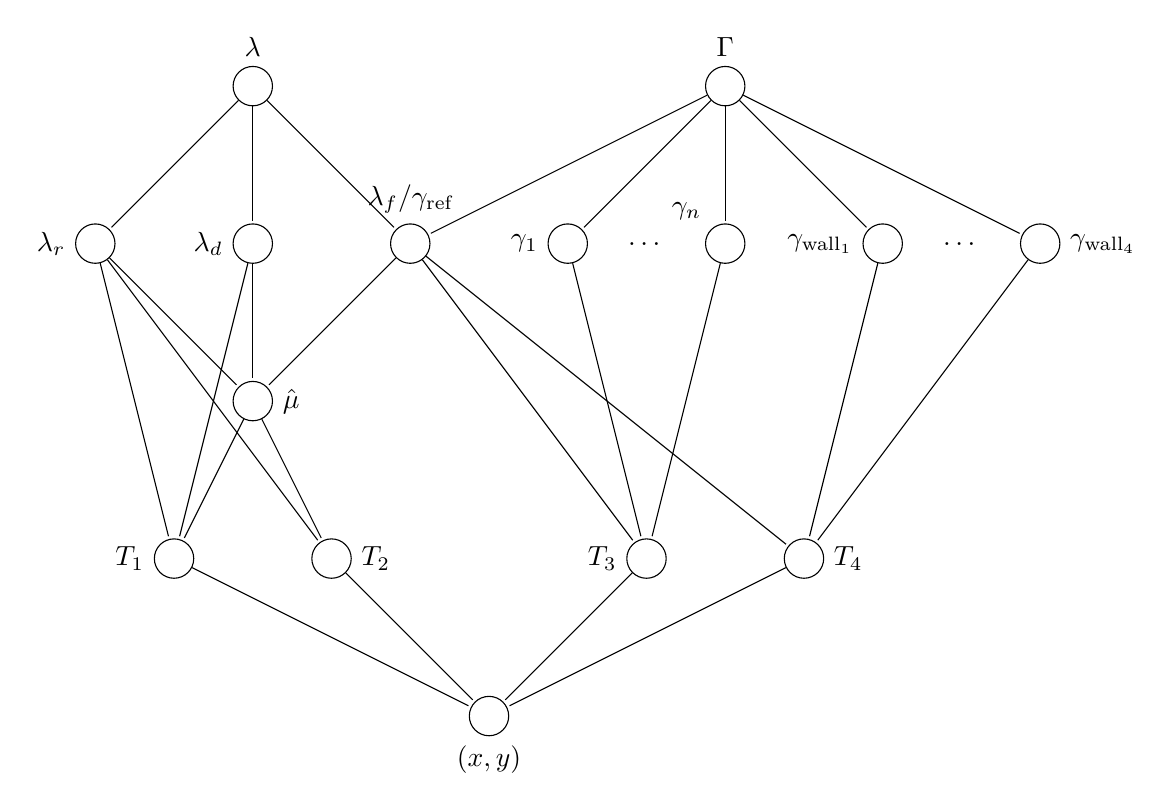
\begin{tikzpicture}[-, >=stealth', shorten >=1pt, auto, node distance=2cm, every state/.style={fill=white, draw=black, text=black, minimum size=0.5cm}]
	\node[state, label=above:$\lambda$] (cmd) {};
	\node[state, label=above:$\Gamma$] (world) [right of=cmd, xshift=4cm] {};
	\node[state, label=left:$\lambda_d$] (dist) [below of=cmd] {};
	\node[state, label=left:$\lambda_r$] (dir) [left of=dist] {};
	\node[state, label=above:$\lambda_f/\gamma_{\refobj}$] (ref) [right of=dist] {};
	\node[state, label=left:$\gamma_1$] (obj1) [below of=world, xshift=-2cm] {};
	\node[state, label=above left:$\gamma_n$] (objn) [right of=obj1] {};
	\node[state, label=left:$\gamma_{\textmd{wall}_1}$] (wall1) [right of=objn] {};
	\node[state, label=right:$\gamma_{\textmd{wall}_4}$] (wall4) [right of=wall1] {};
	\node[state, label=right:$\hat{\mu}$] (mu) [below of=dist] {};
	\node[state, label=left:$T_1$] (t1) [below of=mu, xshift=-1cm] {};
	\node[state, label=right:$T_2$] (t2) [right of=t1] {};
	\node[state, label=left:$T_3$] (t3) [right of=t2, xshift=2cm] {};
	\node[state, label=right:$T_4$] (t4) [right of=t3] {};
	\node[state, label=below:${(x, y)}$] (pt) [below of=t2, xshift=2cm] {};
	
	\path (cmd) edge (dist)
	         (cmd) edge (dir)
	         (cmd) edge (ref)
	         (world) edge (ref)
	         (world) edge (obj1)
	         (world) edge (objn)
	         (world) edge (wall1)
	         (world) edge (wall4)
	         (obj1) -- node[auto=false]{\ldots} (objn)
	         (wall1) -- node[auto=false]{\ldots} (wall4)
	         (dir) edge (mu)
	         (dist) edge (mu)
	         (ref) edge (mu)
	         (dir) edge (t1)
	         (dir) edge (t2)
	         (dist) edge (t1)
	         (mu) edge (t1)
	         (mu) edge (t2)
	         (ref) edge (t3)
	         (ref) edge (t4)
	         (obj1) edge (t3)
	         (objn) edge (t3)
	         (wall1) edge (t4)
	         (wall4) edge (t4)
	         (t1) edge (pt)
	         (t2) edge (pt)
	         (t3) edge (pt)
	         (t4) edge (pt);


\end{tikzpicture}
\end{center}

\section*{Putting the Model Together}
Given these features, we obtain the log-linear model
\[
\mathbb{P}_w(x, y|\lambda, \Gamma) = \frac{1}{z_w(\lambda, \Gamma)}\exp\bigg(\sum_{c = 1}^4w_cT_c(x, y|\lambda, \Gamma)\bigg)
\]
where $w$ is a vector of weights. We then learn the weights using MLE estimation.

\subsection*{MLE Estimation for Learning Weights}
We trained the model using the data from scene \#1. We assume each data point is an iid sample from $\prob_w(x, y|\lambda, \Gamma)$. Let the 12 commands be specified by $\lambda^{(1)}, \ldots, \lambda^{(12)}$. For each command we collected 10 data points. Let $X$ represent all the data and let $X^{(i)}_j$ be the $j$-th data point for the $i$-th command. Then the joint probability of the data points can be expressed as

\begin{equation*}
\begin{split}
\prob_w(X|\lambda^{(1)}, \ldots, \lambda^{(12)}, \Gamma) &= \prod_{i = 1}^{12}\prod_{j = 1}^{10} \frac{1}{z_w(\lambda^{(i)}, \Gamma)}\exp\bigg(\sum_{c = 1}^4w_cT_c(X^{(i)}_j|\lambda^{(i)}, \Gamma)\bigg) \\
&= \bigg(\prod_{i = 1}^{12}\prod_{j = 1}^{10} \frac{1}{z_w(\lambda^{(i)}, \Gamma)}\bigg)\bigg(\prod_{i = 1}^{12}\prod_{j = 1}^{10}\exp\bigg(\sum_{c = 1}^4w_cT_c(X^{(i)}_j|\lambda^{(i)}, \Gamma)\bigg)\bigg) \\
&= \bigg(\prod_{i = 1}^{12}\prod_{j = 1}^{10} \frac{1}{z_w(\lambda^{(i)}, \Gamma)}\bigg)\exp\bigg(\sum_{c = 1}^4w_c\sum_{i = 1}^{12}\sum_{j = 1}^{10}T_c(X^{(i)}_j|\lambda^{(i)}, \Gamma)\bigg)
\end{split}
\end{equation*}

Our goal then is to find the argmax over $w$ of this function. This is the same as finding the argmin of the negative log, so we have
\begin{equation*}
\begin{split}
w^* &= \argmin_w -\log\prob_w(X|\lambda^{(1)}, \ldots, \lambda^{(12)}, \Gamma) \\
&= \argmin_w \sum_{i = 1}^{12}\sum_{j = 1}^{10}\log(z_w(\lambda^{(i)}, \Gamma)) - \sum_{c = 1}^4w_c\sum_{i = 1}^{12}\sum_{j = 1}^{10}T_c(X^{(i)}_j|\lambda^{(i)}, \Gamma)
\end{split}
\end{equation*}

This is the sum of exponential families, one for each $i, j$. Therefore the derivative with respect to $w_c$ of the log partition function is the expected value of the $c$-th feature. Therefore, 
\[
\frac{\partial}{\partial w_c} -\log\prob_w(X|\lambda^{(1)}, \ldots, \lambda^{(12)}, \Gamma) = \sum_{i = 1}^{12}\sum_{j = 1}^{10} \E_w[T_c(x, y|\lambda^{(i)}, \Gamma)] - \sum_{i = 1}^{12}\sum_{j = 1}^{10}T_c(X^{(i)}_j|\lambda^{(i)}, \Gamma)
\]

We use this to perform gradient descent. In order to calculate the probabilities and the partition function, we discretize the table with a grid of step size 0.1 inches. Once we do this, we have all the components necessary to calculate the gradient, and so we perform gradient descent until the gradient falls below a threshold level.

\section*{Modeling Results}

\end{document}